%%%%%%%%%%%%%%%%%%%%%%%%%%%%%%%%%%%%%%%%%%%
%%% DOCUMENT PREAMBLE %%%
\documentclass[12pt]{article}

\usepackage{agda}
\usepackage{apacite}
\usepackage{catchfilebetweentags}

\usepackage{ucs}
\usepackage{amssymb}

\usepackage[english]{babel}
\usepackage{url}
\usepackage[utf8x]{inputenc}
\usepackage{amsmath}
\usepackage{graphicx}
\graphicspath{{images/}}
\usepackage{parskip}
\usepackage{fancyhdr}
\usepackage{vmargin}
\setmarginsrb{3 cm}{2.5 cm}{3 cm}{2.5 cm}{1 cm}{1.5 cm}{1 cm}{1.5 cm}

\title{Programming a cryptocurrency in Agda}								

% Title
\author{Guilherme H. A. Silva}						
% Author
\date{15 de Abril de 2019}
% Date

\makeatletter
\let\thetitle\@title
\let\theauthor\@author
\let\thedate\@date
\makeatother

\pagestyle{fancy}
\fancyhf{}
\rhead{\theauthor}
\lhead{\thetitle}
\cfoot{\thepage}
%%%%%%%%%%%%%%%%%%%%%%%%%%%%%%%%%%%%%%%%%%%%
\begin{document}

%%%%%%%%%%%%%%%%%%%%%%%%%%%%%%%%%%%%%%%%%%%%%%%%%%%%%%%%%%%%%%%%%%%%%%%%%%%%%%%%%%%%%%%%%

\begin{titlepage}
	\centering
    \vspace*{0.5 cm}
   % \includegraphics[scale = 0.075]{bsulogo.png}\\[1.0 cm]	% University Logo
   \begin{center}    \textsc{\Large   Fundação Getúlio Vargas}\\[2.0 cm]	\end{center}% University Name
   \textsc{\Large Modelagem Matemática  }\\[0.5 cm]				% Course Code
	\rule{\linewidth}{0.2 mm} \\[0.4 cm]
	{ \huge \bfseries \thetitle}\\
	\rule{\linewidth}{0.2 mm} \\[1.5 cm]
	
	\begin{minipage}{0.4\textwidth}
		\begin{flushleft} \large
		%	\emph{Submitted To:}\\
		%	Name\\
          % Affiliation\\
           %contact info\\
			\end{flushleft}
			\end{minipage}~
			\begin{minipage}{0.4\textwidth}
            
			\begin{flushright} \large
        \emph{Student:} \\
        Guilherme Horta Alvares da Silva \\
        \emph{Professor:} \\
        Doctor Flávio Codeço Coelho
		\end{flushright}
           
	\end{minipage}\\[2 cm]

  \includegraphics[scale = 0.5]{imgs/FGV.png}
    
	
\end{titlepage}

%%%%%%%%%%%%%%%%%%%%%%%%%%%%%%%%%%%%%%%%%%%%%%%%%%%%%%%%%%%%%%%%%%%%%%%%%%%%%%%%%%%%%%%%%

\tableofcontents
\pagebreak

%%%%%%%%%%%%%%%%%%%%%%%%%%%%%%%%%%%%%%%%%%%%%%%%%%%%%%%%%%%%%%%%%%%%%%%%%%%%%%%%%%%%%%%%%
\renewcommand{\thesection}{\arabic{section}}
\section{Introduction}

\subsection{Cryptocurrencies}

In 1983, David Chaum created ecash \cite{panurach1996money} , an anonymous cryptographic eletronic money.
This cryptocurrency use RSA blind signatures \cite{chaum1983blind} to spend transactions.
Later, in 1989, David Chaum found an eletronic money corporation called DigiCash Inc.
It was declared bankruptcy in 1998.

Adam Back developed a proof-of-work (PoW) scheme for spam control, Hashcash \cite{back2002hashcash}.
To send an email, the hash of the content of this email plus a nounce has to have a numerically value smaller than a defined target.
So, to create a valide email, the sender (miner) has to spend a considerable CPU resource on it.
Because, hash functions produces pratically random values, so the miner has to guess a lot of nounce values before find some nounce that make the hash of the email less than the target value.
This idea is the same that is used in Bitcoin proof of work, because each block has a nounce guessed by the miner and the hash of the block has to be less than the target value.

Wei Dai propose b-money \cite{dai1998b} for the first proposal for distributed digital scarcity.
And Hal Finney created Bit Gold, a reusable proof of work for hashcash for its algorithm of proof of work.

In 31 October 2008, Satoshi Nakamoto registered the website ``bitcoin.org'' and put a link for his paper \cite{nakamoto2008bitcoin} in a cryptography mailing list.
In January 2009, Nakamoto released the bitcoin software as open-source code.
The identity of Satoshi Nakamoto is still unknown.
Since that time, the total market of Bitcoin came to 330 billions dollars in 17 of December of 2018
and his value has a historic record of 20 thousands dollars.

Other cryptocurrencies like Ethereum \cite{wood2014ethereum}, Monero \cite{noether2015ring} and ZCash \cite{hopwood2016zcash} were created after Bitcoin,
but Bitcoin is still the cryptocurrency with the biggest market value.

Ethereum is a cryptocurrency that uses account model instead of UTXO used in bitcoin for its transaction data struct.
It uses Solidity as its programming language for smart contracts, it looks like Java Script,
so it is easier to programming in it than in stack machine programming language of Bitcoin.
Ethereum is now changing from proof of work (used in Bitcoin) to proof of stake.

Monero and ZCash are both cryptocurrency that focus on fungibility, privacy and descentralization.
Monero uses obfuscated public ledger, so anyone can send transcations, but nobody can tell the source, amount or destination.
Zcash uses the concept of zero-knowledge proof called zk-SNARKs, which garantee privacy for its users.

\subsection{Bitcoin}

The bitcoin was made to be a peer to peer eletronic cash.
It was made in one way that users can save and verify transactions without the need of a trust party.
Because of that no authority or goverment can block the bitcoin.

Transactions in bitcoins are one array of input of previous transactions and one array of outputs.
The mining transaction does not need to have an input.
For each input of the transaction, it is necessary a signature signed with a private key to prove the ownerchip of the bitcoins.

Transactions are grouped in a block.
Each block has in its header the timestamp that the block was created, the hash of the block,
the previous hash and a nounce.
A nounce is an arbitrary value that the miner has to choose to make the hash of the block respect some specific characteristics.

Each block has a limit size of 1 MB.
Because of that, bitcoin has a blockchain (one array of blocks).
Each block should be created in an average of 10 minutes.
This time was choosen because in 10 minutes, it is enough to propagate the block in all the world.
To make it possible, there is a concept called proof of work in bitcoin.
So the miner has choose a random value as nounce that makes the hash of the block less than a certain value.
This value is choosen in a way that each block should be generated in 10 minutes in average.
If the value is too low, miners will take more time to find a nounce that make the hash block less than the it.
If it is too high, it will be easier to find a nounce and they will find it faster.

When two blocks are mined in nearly the same time, there are two valid blockchains.
It is because the last block in the both blockchains are valid but different.
Because of this problem, in Bitcoin protocol, the largest chain is always the right chain.
While two valid chains have the same size, it is not possible to know which chain is the right.
This situation is called fork and when it happens, it is necessary to wait to see in which chain the new block will be.

In Bitcoin, there is a possibility of 51% attack.
It happens when some miner, with more power than all network, mine secretly the blocks.
So if the main network has 50 blocks, the miner could produce hidden blocks from 46 to 55
and he would have 10 hidden blocks from the network.
When he shows their hidden blocks, his chain become the valid chain, because it is bigger.
So all transactions from previous blockchain from 46 to 50 blocks become invalid.
Because of that, when someone make a big transaction in the blockchain, it is a good idea to wait more time.
So it is becoming harder and harder to make a 51% with more time.
Bitcoin has the highest market value nowadays, so attacking the bitcoin network is very expensive.
Nowadays, this kind of attack is more common in new altcoins.

\subsection{Ethereum}

Ethereum differs from bitcoin in having an Ethereum Virtual Machine (EVM) to run script code.
EVM is a stack machine and turing complete while Bitcoin Script is not
(it is impossible to do loops and recursion in Bitcoin).

Transactions in bitcoin are all stored in blockchain.
In Ethereum, just the hash of it is stored in it.
So it is saved in off chain database.
Because of that, it is possible to save more information in Ethereum Blockchain.

In Bitcoin, the creator of the contract as to pay the amount proportional to its size.
But in Ethereum, every time the user run a contract that change some data,
he has to pay some gas for it.
Each instruction in EVM has a fixed amount of gas pre defined that is necessary to pay.
The user must set how much ether he wants to pay per gas.
So if the user stays without ether, the contract halt and stopped to being executed.

Because Ethereum has its own EVM with more instructions than Bitcoin and it is Turing Complete,
its considered less secure.
Ethereum has its own high level programming language called Solidity that looks like JavaScript.

\subsection{Introduction}

Before my work, there were some research in this field.
Antom Setzel already code the definitions of transactions and transactions tree of bitcoin.
Orestis Melkonian start to formalize Bitcoin Script.

My work try to extend Antom Setzel model and make possible to use Bitcoin protocol
from inputs and outputs from plain text.
For example, the user send a transaction in plain text to the software and it validates if it is right.
To use the Antom Setzel model, the user has to send the data and the proof that it is correct.

\subsection{Agda Introduction}
Agda is a dependently typed functional language developed by Norell at Chalmers University of Technology as his PhD Thesis.
The current version of Agda is Agda 2.

  \subsection{Martin-Löf type theory}
  Agda is also a proof assistance based on intensional Martin-Löf type theory.

    \subsection{Types}
    In Martin-Löf type theory, there are 3 finites types and 5 types constructors.
    The 0 type contain 0 terms, it is called empty type and it is written bot.
    \ExecuteMetaData[latex/agdaExamples.tex]{botType}

    The 1 type is the type with just 1 canonical term and it represents existence.
    It is called unit type and it is written top .
    \ExecuteMetaData[latex/agdaExamples.tex]{trivialType}

    The 2 type contains 2 canonical terms. It represents a choice between two values.
    \ExecuteMetaData[latex/agdaExamples.tex]{eitherType}

    The Boolean Type is defined using the Trivial type and the Either type
    \ExecuteMetaData[latex/agdaExamples.tex]{boolType}

    If statement is defined using booleans
    \ExecuteMetaData[latex/agdaExamples.tex]{ifThenElse}

    \subsection{Types Constructors}
    The sum-types contain an ordered pair.
    The second type can depend on the first type.
    It has the same meaning of exist.
    \ExecuteMetaData[latex/agdaExamples.tex]{sumType}

    The pi-types contain functions.
    So given an input type, it will return an output type.
    It has the same meaning of a function
    \ExecuteMetaData[latex/agdaExamples.tex]{piType}

    In Inductive types, it is a self-referential type.
    Naturals numbers are examples of that
    \ExecuteMetaData[latex/agdaExamples.tex]{Nat}
    Other data structs like linked list of natural numbers, trees, graphs are too.
    Proofs in inductive types are made by induction.
    \ExecuteMetaData[latex/agdaExamples.tex]{NatElim}

    Universe types are created to allow proofs written in all types.
    For example, the type of Nat is U0.


It looks like CoQ, but does not have tatics.
Agda is a total language, so it is garanteed that the code always terminal and coverage all inputs.
Agda needs it to be a consistent language.

Agda has inductive data types that are similar to algebric data types in non-depently typed programming language.
The definition of Peano numbers in Agda:

\ExecuteMetaData[latex/agdaExamples.tex]{Nat}

Definitions in Agda are done using induction.
For example, the sum of two numbers in Agda:

\ExecuteMetaData[latex/agdaExamples.tex]{sum}

In Agda, because of dependent types, it is possible to make some restrictions in types that is not possible in other language.
For example, get the first element of a vector.
For it, it is necessary to specify in the type that the vector should have at size greater or equal tha than one.

\ExecuteMetaData[latex/agdaExamples.tex]{vecHead}

Another good example is that in sum of two matrices, they should have the same dimentions.

\ExecuteMetaData[latex/agdaExamples.tex]{matrixSum}

\subsection{UTXO Bitcoin}

There are two kinds of data structures to modeling accounts records and savings states.
The UTXO model used in Bitcoin and the account model used in Ethereum.

  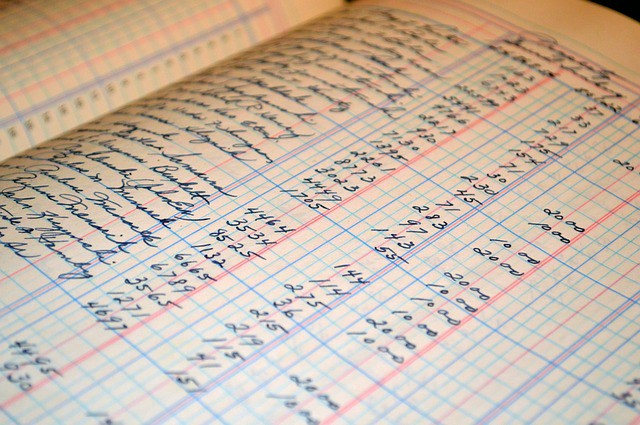
\includegraphics[scale = 0.7]{imgs/account.jpeg}

In account model, it is saved the address and the balance of each address.
For example, the data struct will look like this [(0xabc01, 1.01), (0xabc02, 2.02)].
So the address 0xabc01 has 1.01a of balance and the address 0xabc02 has 2.02 of balance.
In this way, it is possible to easily know how much of balance each address has,
but it is not possible to know how they got in this state.

  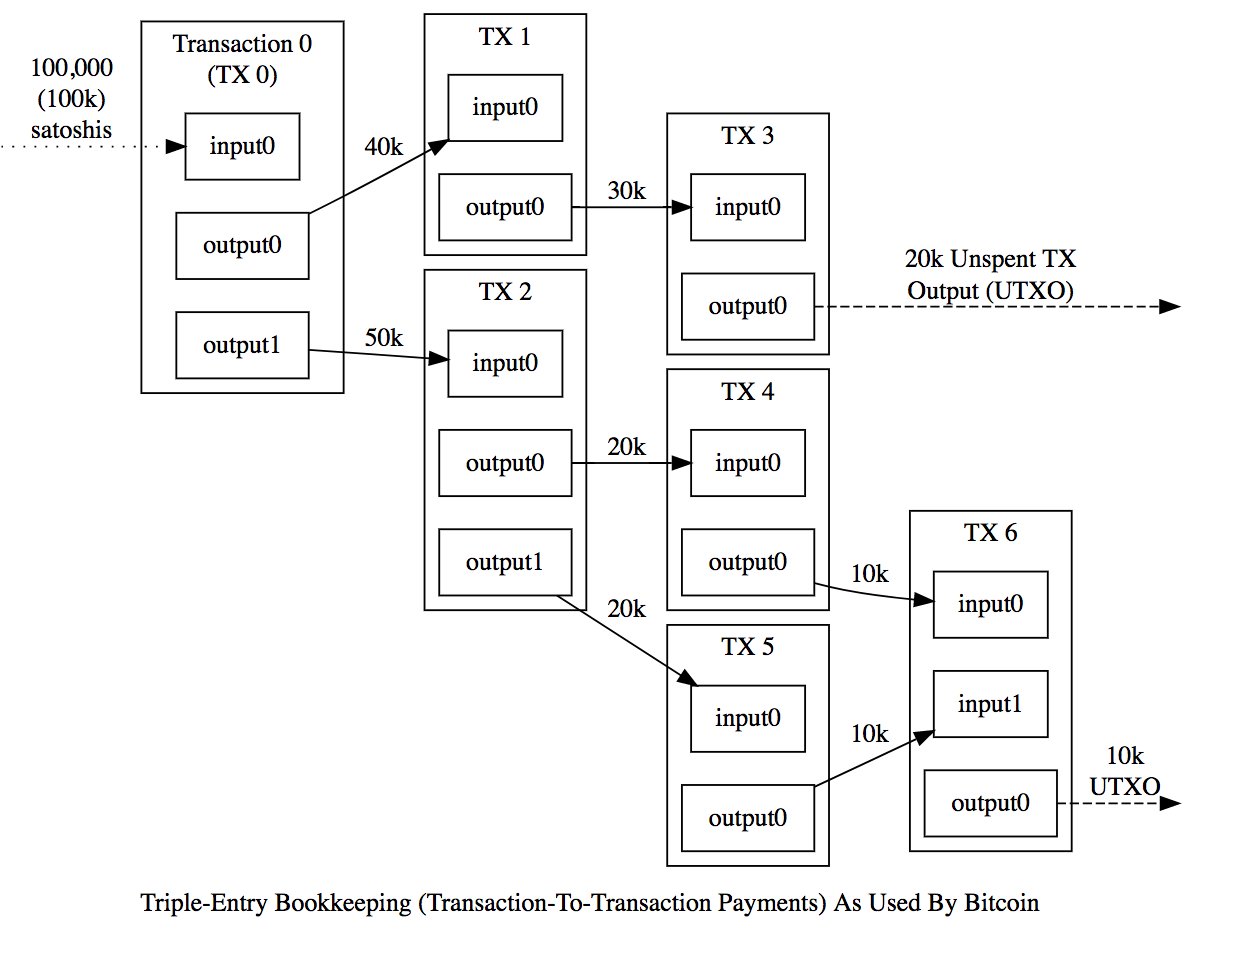
\includegraphics[scale = 0.4]{imgs/utxo.png}

In UTXO model, each transaction is saved in the transaction tree.
Every transaction is composed of multiples inputs and multiples outputs.
But all inputs have to never been spent before.

Because of that, in UTXO model, it is easy to make a new transaction from previous one, but it is harder to know how much each one has.
The wallet that calculate how much balance each address has.

In account model, there could be one kind of vulnerability that is less probabable to happen in UTXO model.
Because there is an undesirable intermediary state that there is some address without balance while another has not already received his money.

For example: \\
bobBalance -= 1 \\
Intermediary State \\
aliceBalance += 1

In account model, it is straight foward to know how much balance each address has.
In UTXO model, this calculation is made offchain. It can be a good thing,
because each user has more privacy.

\subsection{TXTree in Agda}

\section{Methods}

\subsection{Cripto Functions}
The first thing that we define are the cripto functions that will be needed to make the cripto currency.
Message can be defined in multiple ways, one array of bytes, one string or a natural number.
Message in this context means some data.

Private key is a number, a secret that someone has.
In Bitcoin, the private key is a 256-bit number.
Private key is used to signed messages.

Public key is generated from private key.
But getting private key from public key is impossible.
To verify who signed a message with a private key, he has to show the public key.

Hash is an injection function (the probability of collision is very low).
The function is used from a big domain to a small domain.
For example, a hash of big file (some GBs) is an integer of just some bytes.
It is very usefull to prove for example that 2 files are equal.
If the hash of two files are equal, so the files are equal.
It is used in torrents clients, so it is safe to download a program to untrusted peers,
just have to verify if the hash of the file is equal to the hash of the file wanted.

These functions can be defined, but it is not the purpose of this theses.
So they will be just postulates.

\ExecuteMetaData[latex/Cripto.tex]{criptoPostulates}

\section{Conclusion}

\newpage
 
\bibliographystyle{apacite}
\bibliography{References}

\end{document}
